\documentclass[tikz,border=5mm]{standalone}
\usepackage[T1]{fontenc}
\usepackage{helvet}
\renewcommand{\familydefault}{\sfdefault}
\usepackage[helvet]{sfmath}
\usepackage{tikz}
\usetikzlibrary{arrows.meta, calc, decorations.markings}

\begin{document}
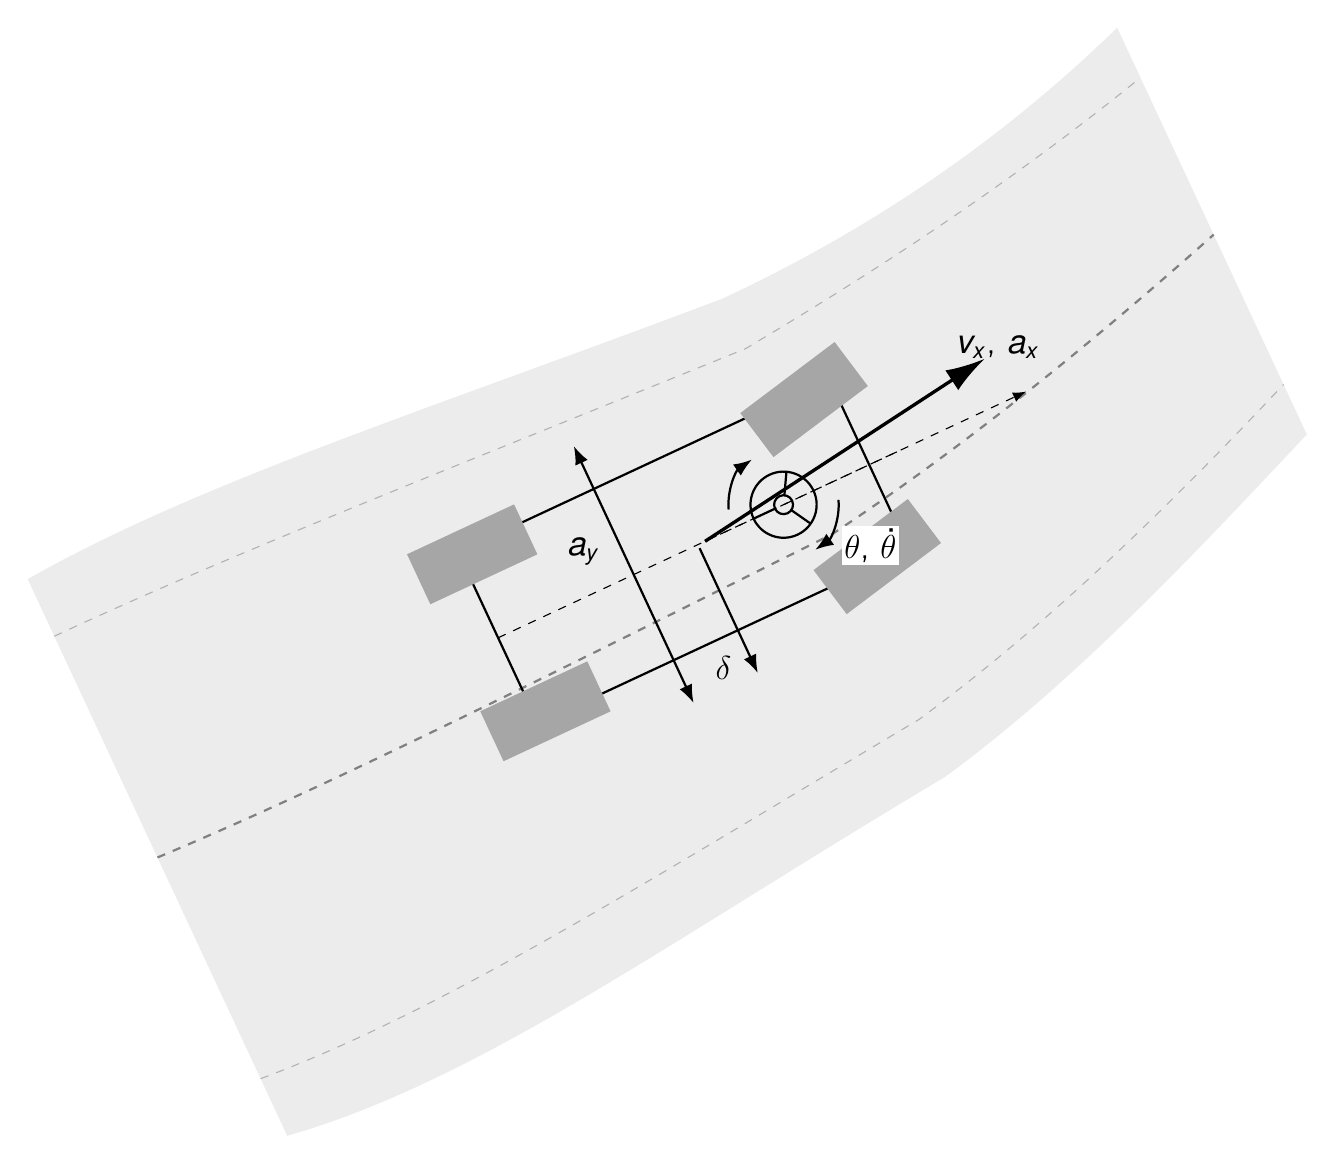
\begin{tikzpicture}[>=Latex]

%% ============================================================
%% Global rotation: the whole car+road scene is rotated ~25 deg
%% ============================================================
\def\roadAngle{25}

\begin{scope}[rotate=\roadAngle]

%% ---- Road ----
%% Curved road as a filled region (light gray)
\fill[gray!15]
  (-6.5, -3.8) .. controls (-4,-4.2) and (-1,-3.6) ..
  (3, -3.2) .. controls (5,-2.8) and (7,-2.0) ..
  (9, -1.2)
  -- (9, 4.5) .. controls (7,3.8) and (5,3.5) ..
  (3, 3.5) .. controls (-1,3.8) and (-4,4.2) ..
  (-6.5, 4.0) -- cycle;

%% Road centre line (dashed)
\draw[gray, dashed, thick]
  (-6.5, 0.1) .. controls (-4,0.0) and (-1,0.1) ..
  (3, 0.2) .. controls (5,0.5) and (7,1.0) ..
  (9, 1.6);

%% Road edge lines (dashed, lighter)
\draw[gray!60, dashed]
  (-6.5, -3.0) .. controls (-4,-3.2) and (-1,-2.8) ..
  (3, -2.4) .. controls (5,-2.0) and (7,-1.3) ..
  (9, -0.5);
\draw[gray!60, dashed]
  (-6.5, 3.2) .. controls (-4,3.2) and (-1,3.0) ..
  (3, 2.8) .. controls (5,3.0) and (7,3.3) ..
  (9, 3.8);

%% ---- Car body (rectangle) ----
\def\carW{2.6}   % half-width (longitudinal)
\def\carH{1.2}   % half-height (lateral)
\coordinate (C) at (1.2, 0.8);  % car centre

\draw[thick] ($(C)+(-\carW,-\carH)$) rectangle ($(C)+(\carW,\carH)$);
%% dashed longitudinal axis of car
\draw[thin, dashed] ($(C)+(-\carW,0)$) -- ($(C)+(\carW+0.4,0)$);

%% ---- Wheels (filled gray rectangles) ----
\def\wW{0.75}  % wheel half-width
\def\wH{0.35}  % wheel half-height

% Rear left
\fill[gray!70] ($(C)+(-\carW+0.15, \carH-0.1)+(-\wW,-\wH)$)
  rectangle ($(C)+(-\carW+0.15, \carH-0.1)+(\wW,\wH)$);
% Rear right
\fill[gray!70] ($(C)+(-\carW+0.15,-\carH+0.1)+(-\wW,-\wH)$)
  rectangle ($(C)+(-\carW+0.15,-\carH+0.1)+(\wW,\wH)$);

% Front wheels – rotated by steering angle (~12 deg)
\def\steerAng{12}
\begin{scope}[shift={($(C)+(\carW-0.4, \carH-0.1)$)}, rotate=\steerAng]
  \fill[gray!70] (-\wW,-\wH) rectangle (\wW,\wH);
\end{scope}
\begin{scope}[shift={($(C)+(\carW-0.4,-\carH+0.1)$)}, rotate=\steerAng]
  \fill[gray!70] (-\wW,-\wH) rectangle (\wW,\wH);
\end{scope}

%% ---- Velocity arrow  v_x, a_x  (thick, along heading) ----
\draw[-{Latex[length=5mm,width=3mm]}, very thick]
  ($(C)+(0.3,0)$) -- ($(C)+(4.5, 0.6)$);
%% thin dashed arrow along car longitudinal axis
\draw[-{Latex}, thin, dashed] ($(C)+(0.3,0)$) -- ($(C)+(4.8,0)$);

%% Label v_x, a_x
\node[anchor=south west, font=\large] at ($(C)+(4.0, 0.7)$)
  {$v_x$, $a_x$};

%% ---- Lateral acceleration  a_y  (double-headed arrow, perpendicular) ----
\draw[{Latex}-{Latex}, thick]
  ($(C)+(-0.7, -\carH-0.6)$) -- ($(C)+(-0.7, \carH+0.6)$);
\node[anchor=east, font=\large] at ($(C)+(-0.85, 0.4)$) {$a_y$};

%% ---- Steering angle  δ  (short arrow below front-left area) ----
\draw[-{Latex}, thick]
  ($(C)+(0.2, -0.05)$) -- ($(C)+(0.2, -\carH-0.6)$);
\node[anchor=north east, font=\large] at ($(C)+(0.15, -\carH-0.2)$)
  {$\delta$};

%% ---- Steering wheel symbol  (circle with spokes) ----
\coordinate (SW) at ($(C)+(1.4, 0)$);
\draw[thick] (SW) circle (0.42cm);
\draw[thick] (SW) circle (0.12cm);
% spokes
\foreach \a in {60,180,300} {
  \draw[thick] ($(SW)+({\a}:0.12)$) -- ($(SW)+({\a}:0.42)$);
}

%% ---- Yaw angle  θ, θ̇  (curved arrows near steering wheel) ----
\draw[-{Latex}, thick] ($(SW)+(160:0.7)$) arc (160:100:0.7);
\draw[-{Latex}, thick] ($(SW)+(-20:0.7)$) arc (-20:-80:0.7);
\node[anchor=north west, font=\large, fill=white, inner sep=1pt] at ($(SW)+(0.55, -0.55)$)
  {$\theta$, $\dot{\theta}$};

\end{scope}

\end{tikzpicture}
\end{document}
